\chapter{Theory}
In this chapter the fundamental physics behind the Hall effect will be discussed. The Hall coefficient and charge carrier density will also be discussed. These both are unique material properties, which are related to each other. How so will become clear at the end of this chapter.

\section{The Hall effect}
When an electric current $I$ flows through a conductor perpendicular to a magnetic field $B$, it results in a transverse force $F_m$ on the moving charge carriers due to the magnetic field. Those charge carriers are pushed to one side of the conductor due to the Hall effect. All the chargers are building up at one side of the conductor. Because of this, there is a measurable voltage difference between the two sides of the conductor. This measurable voltage difference is called the Hall voltage. This Hall voltage is due is a potential difference due to the Hall effect. This effect is called after E.H. Hall, who discovered the Hall effect in 1897 [bron?]. The change in the direction of the current $I$ is caused by the magnetic force. This force is given by [bron?]:
    \begin{equation}
        \vec F = q\cdot (\vec E + \vec v \times \vec B)
        \label{eq:force}
    \end{equation}
%   
    \begin{table}[!htbp]
    \centering
    \caption{The quantities belonging to Equation \ref{eq:force}.}
    \label{table:force}
    \begin{tabular}{|c|c|c|}
    \hline
    \textbf{Quantity}   & \textbf{Description}           & \textbf{Unit}            \\ \hline
    $q$                  & Electrical charge    & {[}C{]}                     \\ \hline
    $\vec E$                  & Electric field strength         & {[}V/m{]}                     \\ \hline
    $\vec v$                  & Drift speed           & {[}m/s{]}                     \\ \hline
    $\vec B$                  & Magnetic field & {[}T{]} \\ \hline
    \end{tabular}
    \end{table}
    \begin{figure}[!htbp]
    \begin{center}
        \begin{minipage}[t]{0.45\textwidth}
            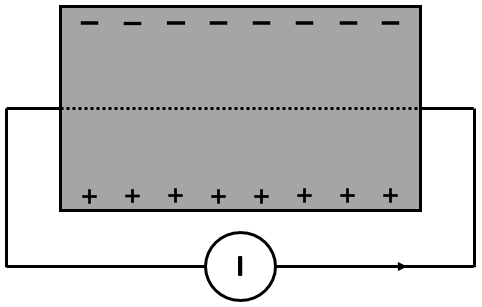
\includegraphics[scale=0.45]{figuren/theorie_e_rechtdoor.png}
            \caption{A schematic of the coil configuration.} \label{fig:schematic_setup_magnets}
        \end{minipage}
        \begin{minipage}[t]{0.45\textwidth}
            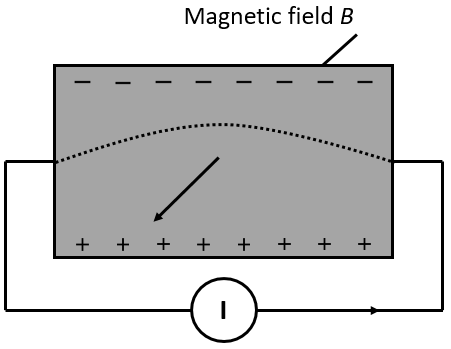
\includegraphics[scale=0.47]{figuren/theorie_e_afbuigen.png}
             \caption{The schematic setup for the experimental setup of the Hall effect.}\label{fig:schematic_hall_effect}
        \end{minipage}
    \end{center}
    \end{figure}
\begin{figure} [!htbp]
    \centering
    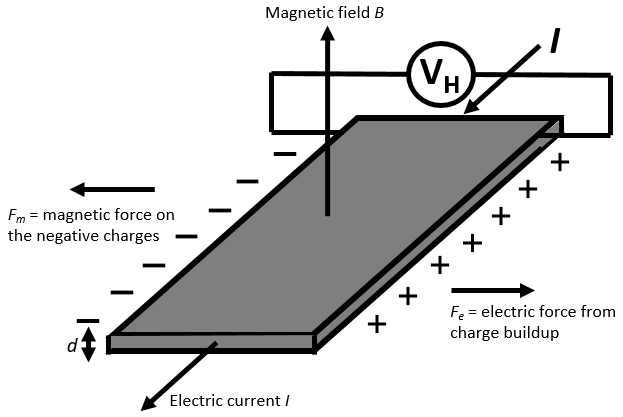
\includegraphics[scale=0.7]{figuren/schematic_forces.png}
    \caption{A schematic representation of the force on a current due to the Hall effect.}
    \label{fig:schematic_force}
\end{figure}
The quantities belonging to Equation \ref{eq:force} are defined in Table \ref{table:force}.
Because of this force, the positive and negative charges will have an acceleration in the direction of the force. This results in a change of the path of the charges. Which will lead to a potential difference.\\
Without magnetic field and thus without the force, the charges will go straight from one side of the material to the other, see Figure \ref{fig:schematic_setup_magnets}. When there is a magnetic field, the path changes in a curve, see Figure \ref{fig:schematic_hall_effect}. The potential different due to this effect is called the Hall Voltage. The Hall voltage is given by:
    \begin{equation}
        U_H = v_d\cdot B \cdot d
        \label{eq:Hall voltage}
    \end{equation}
With the distance $d$ between the positive and negative side of the plate. 
There also is current of the electrical charge in the negative direction with respect to the electon current, this is the conventional 'hole' current. This current can be written as:
    \begin{equation}
        I_x = n\cdot tw\cdot (-v_d)\cdot (-e)
        \label{eq:Hole current}
    \end{equation}
The quantities belonging to Equation \ref{eq:Hole current} are defined in Table \ref{table:Hole current}.
    \begin{table}[!htbp]
    \centering
    \caption{The quantities belonging to Equation \ref{eq:Hole current}.}
    \label{table:Hole current}
    \begin{tabular}{|c|c|c|}
    \hline
    \textbf{Quantity}   & \textbf{Description}           & \textbf{Unit}            \\ \hline
    $n$                  & Charge carrier density    & {[}Electrons/m^3{]}                     \\ \hline
    $tw$                  & The cross-sectional area         & {[}m^2{]}                     \\ \hline
    $-v_d$                  & Drift speed           & {[}m/s{]}                     \\ \hline
    $-e$                  & Charge of each electron & {[}C{]} \\ \hline
    \end{tabular}
    \end{table}
In which $e$ is the elementary charge, being equal to \cite{elementarycharge}:
\begin{equation}
    e = (1.602... \cdot 10^{-19} \pm 6.1 \cdot 10^{-9}) \quad \text{[C]} \label{eq:e}
\end{equation}
This equation can be solved for \emph{w} and plugged into Equation \ref{eq:Hall voltage} resulting in the Hall voltage:
 \begin{equation}
        U_H = \frac{1}{n \cdot e} \frac{B \cdot I}{d}. \label{eq:Hall Voltage2}
    \end{equation}

\section{Hall coefficient \& charge carrier density}
The Hall effect can be used to determine the Hall coefficient, which is an unique material property. this can be done by writing equation \ref{eq:Hall Voltage2} in the form of
    \begin{equation}
        U_H = R_H \frac{B I}{d} \label{eq:hallspanning_with_coefficient}
    \end{equation}
Where $R_H=\frac{1}{n \cdot e}$ is called the Hall coefficient. For silver $R_H$ is equal to \cite{apparatus_silver}:
    \begin{equation}
        \mid R_H \mid = (8,9 \pm 2) \cdot 10^{-11}  \quad \text{[m$^3$C$^{-1}$]} \label{eq:hallcoefficient_lit}
    \end{equation}
When the electric charge of the charge carriers in a material is known, Equation \ref{eq:hallspanning_with_coefficient} can be used to determine the charge carrier density. The charge carrier density $n$ is the number of charge carriers per volume.  The charge carrier density denotes the number of charge carriers per volume. It is measured in m$^{-3}$. As any density it can depend on position. It should not be confused with the charge density, which is the number of charges per volume at a given energy [bron?]. The charge carrier density is received by rewriting Equation \ref{eq:Hall Voltage2} to:
    \begin{equation}
        n = \frac{1}{e} \cdot \frac{1}{R_H}
    \end{equation}
In which $R_H$ is the Hall coefficient and $e$ the elementary charge. The charge carrier density cannot be directly measured. Therefor it has to be experimentally determined. This can be done by using the Hall effect. Silver for example has a charge carrier density of \cite{apparatus_silver}:
    \begin{equation}
        n = (6.6 \pm 2)\cdot 10^{28} \quad \text{[m$^{-3}$]} \label{eq:ccdensity_lit}
    \end{equation}
It is important to note that the uncertainties of Equation \ref{eq:hallcoefficient_lit} and Equation \ref{eq:ccdensity_lit} are not given by their source. However, their experimental results in comparison with the literature value are given. The difference between these two have been chosen as the uncertainties for Equation \ref{eq:hallcoefficient_lit} and Equation \ref{eq:ccdensity_lit}.